\section{通配符}\label{sec:通配符}
\sectionAuthor{Jiaqi Z.}

% 请在下方的item内填写本节知识点
\begin{Abstract}
    \item 什么是通配符
    \item 如何使用通配符批量处理文件
\end{Abstract}

在第\ref{chap:Linux命令行操作}章当中,我们介绍了如何使用Linux的命令行进行简单的操作,如查看文件、对文件和目录进行操作等。同时,在第\ref{chap:文本编辑工具vi和vim}章,我们详细介绍了如何使用vi对文本文件进行编辑。对于绝大多数情况,以上两个章节的内容足够后续的计算任务了。

但“人的本性终究是懒惰的”,在大多数时候,我们可能不希望打开vi后再使用\code{/}这样的命令来查找,而是希望直接在命令行查找我们需要的内容。进一步的,对于更多的文件,有时我们希望同时对这些文件的相同内容进行查找,这时在vi中操作就显得麻烦了。因此,在本章,我们会进一步讨论一些在命令行当中的“进阶操作”,主要是为了能够更方便的处理文件和数据。

\subsection{关于通配符\code{*}, \code{?}}\label{subsec:通配符-关于通配符}

通配符是一种特殊语句,主要有星号(\keyword{*})和问号(\keyword{?}),用来\emph{模糊搜索}。例如,当查找文件时,如果不知道真正的字符,或者希望匹配一系列具有相似模式的文件时,可以使用它来代替一个或多个真正字符。

其中,\code{*}表示\emph{零个或多个任意字符}。例如,使用\code{*.txt}表示文件名最后为\code{.txt}的所有文件,可以是\code{hello.txt}, \code{bye.txt}, \code{roselia.txt}等。

\begin{extend}
    上面的例子实际上就是后缀名的表示方法。它并不是一个很新奇的事情,事实上,在Windows操作系统中,当你在打开或者保存文件时,都可以在下面的“文件类型”中看到这种使用通配符的表示方法(如图\ref{fig:通配符-通配符在Windows操作系统下的应用}所示)

    同时,如果你“思维敏捷”的话,可能会联想到\ref{sec:初窥正则表达式}一节所介绍的正则表达式。事实上,通配符在\emph{某种程度上}也是正则表达式当中的一个特例。

    \begin{figure}
        \centering
        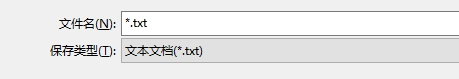
\includegraphics[width=1\linewidth]{Linux基础/高级Linux命令/通配符/fig/通配符.png}
        \caption{通配符在Windows操作系统下的应用}
        \label{fig:通配符-通配符在Windows操作系统下的应用}
    \end{figure}
\end{extend}

相对地,\code{?}表示\emph{零个或一个任意字符},例如,\code{he*o}可以匹配到\code{hello},而\code{he?o}却不能(可以匹配到\code{helo})

\subsection{使用通配符进行文件(目录)操作}\label{subsec:通配符-使用通配符进行文件目录操作}

下面将会简单展示一下,如何使用通配符对文件进行“批量操作”。首先,一个最常见的例子是:批量删除文件。例如,假设当前目录下有\code{data1.dat}和\code{data2.dat}这样两个后缀名为\code{.dat}的文件,如果希望同时删除它们,按照原来的做法,则可能需要按照顺序执行两遍命令:\code{rm data1.dat}和\code{rm data2.dat}。而借助于通配符,可以只使用\code{rm *.dat}表示\emph{删除所有后缀名为\code{.dat}的文件}。

\begin{attention}
    在这一行命令里,通配符所表示的文件可以将其“展开”,等价于\code{rm data1.dat data2.dat}。

    另外,在命令行当中,通配符的优先级比较高,因此,如果一个文件本身含有符号\code{*},则需要使用反斜线(\code{\textbackslash})进行转义,例如,\code{rm \textbackslash*}表示删除当前目录下文件名为\code{*}的文件。相反,使用\code{rm *}表示删除当前目录下所有文件(务必要小心这一命令)
\end{attention}

同样,使用这一方法也可以批量复制文件,与删除类似,可以使用如\code{cp *.dat data}这样的命令将所有后缀名为\code{.dat}的文件复制到\code{data}目录下。

正如前面所说的那样,这一命令可以将其展开成\code{cp data1.dat data2.dat data}

同样,上面对文件名的通配符使用也可以用于目录当中,例如,\code{rm */*.dat}表示删除当前目录下的子目录当中所有后缀名为\code{.dat}的文件。

\begin{attention}
    \code{*}虽然可以表示零个或多个任意字符,但却不能表示\emph{目录下的目录}。例如,\code{rm */data}可以匹配到\code{1/data}, \code{2/data}但无法匹配到\code{1/1/data}这样更深一级的目录。
\end{attention}

关于使用\code{?}通配符的使用方法,其基本原理和使用\code{*}类似,这里不再举例。同时,你也应该意识到的是,上面的例子中,我们都是把通配符放在了开头或者结尾。不一定总是这样的,例如,完全可以使用如\code{hello*.txt}这样的方式表示如\code{hello.txt}, \code{hello1.txt}这样子的文件。

\begin{extend}
    虽然这一套教程是关于Linux的,但在Windows当中,通配符同样十分强大。与我们通常使用Windows的方式不同,它通常是在命令提示符(cmd)当中使用的。如果你希望在Windows当中体验这一功能,可以在开始菜单搜索\code{cmd}(对于新版Windows操作系统也可以是更高级的\code{PowerShell})。

    一些基本的操作语法与Linux类似,但有些操作可能有些许区别。例如,在Windows的命令行当中,使用\code{dir}查看当前目录下的文件,使用\code{del}删除文件,使用\code{copy}复制文件,使用\code{move}移动文件等\footnote{对于cmd命令的完整操作,可以使用cmd下的\code{help}命令查看。}。因此,在Windows当中,可以使用如\code{del *.txt}这样的命令删除当前目录下所有后缀名为\code{.txt}的文件,使用\code{move *.jpg jpg}将当前目录下所有后缀名为\code{.jpg}的文件移动到\code{jpg}目录下。

    这种方式可以有效帮助你批量处理电脑中的文件。
\end{extend}

\subsection{错误处理}\label{subsec:通配符-错误处理}
% 请在本节列出可能遇见的错误与解决方法

\subsubsection{rm: cannot remove <路径名>: No such file or directory}

在\ref{subsec:文件操作-错误处理}一节当中已经介绍了这一错误,但对于通配符的使用而言,这种错误更加常见。例如,上面的例子,当你试着使用通配符\code{*/*.dat}删除\code{1/1/data.dat}文件时,由于无法匹配到对应的文件,因此则会报出这一错误。

\subsubsection{cp: cannot stat <路径名>: No such file or directory}

这一错误与上面的错误类似,都是由于文件不存在所导致的。对于使用通配符的情况,请仔细检查文件名是否正确。